% (find-LATEX "2020-1-C2-def-integral.tex")
% (defun c () (interactive) (find-LATEXsh "lualatex -record 2020-1-C2-def-integral.tex" :end))
% (defun D () (interactive) (find-pdf-page      "~/LATEX/2020-1-C2-def-integral.pdf"))
% (defun d () (interactive) (find-pdftools-page "~/LATEX/2020-1-C2-def-integral.pdf"))
% (defun e () (interactive) (find-LATEX "2020-1-C2-def-integral.tex"))
% (defun u () (interactive) (find-latex-upload-links "2020-1-C2-def-integral"))
% (defun v () (interactive) (find-2a '(e) '(d)) (g))
% (find-pdf-page   "~/LATEX/2020-1-C2-def-integral.pdf")
% (find-sh0 "cp -v  ~/LATEX/2020-1-C2-def-integral.pdf /tmp/")
% (find-sh0 "cp -v  ~/LATEX/2020-1-C2-def-integral.pdf /tmp/pen/")
%   file:///home/edrx/LATEX/2020-1-C2-def-integral.pdf
%               file:///tmp/2020-1-C2-def-integral.pdf
%           file:///tmp/pen/2020-1-C2-def-integral.pdf
% http://angg.twu.net/LATEX/2020-1-C2-def-integral.pdf
% (find-LATEX "2019.mk")

% «.defs»		(to "defs")
% «.title»		(to "title")
% «.exercicio-1»	(to "exercicio-1")
% «.exercicio-2»	(to "exercicio-2")
% «.exercicio-3»	(to "exercicio-3")
% «.def-integral»	(to "def-integral")
% «.def-integral-2»	(to "def-integral-2")
% «.exercicio-4»	(to "exercicio-4")
% «.exercicio-5»	(to "exercicio-5")

\documentclass[oneside,12pt]{article}
\usepackage[colorlinks,citecolor=DarkRed,urlcolor=DarkRed]{hyperref} % (find-es "tex" "hyperref")
\usepackage{amsmath}
\usepackage{amsfonts}
\usepackage{amssymb}
\usepackage{pict2e}
\usepackage[x11names,svgnames]{xcolor} % (find-es "tex" "xcolor")
%\usepackage{colorweb}                 % (find-es "tex" "colorweb")
%\usepackage{tikz}
%
% (find-dn6 "preamble6.lua" "preamble0")
%\usepackage{proof}   % For derivation trees ("%:" lines)
%\input diagxy        % For 2D diagrams ("%D" lines)
%\xyoption{curve}     % For the ".curve=" feature in 2D diagrams
%
\usepackage{edrx15}               % (find-LATEX "edrx15.sty")
\input edrxaccents.tex            % (find-LATEX "edrxaccents.tex")
\input edrxchars.tex              % (find-LATEX "edrxchars.tex")
\input edrxheadfoot.tex           % (find-LATEX "edrxheadfoot.tex")
\input edrxgac2.tex               % (find-LATEX "edrxgac2.tex")
%
%\usepackage[backend=biber,
%   style=alphabetic]{biblatex}            % (find-es "tex" "biber")
%\addbibresource{catsem-slides.bib}        % (find-LATEX "catsem-slides.bib")
%
% (find-es "tex" "geometry")
\usepackage[a6paper, landscape,
            top=1.5cm, bottom=.25cm, left=1cm, right=1cm, includefoot
           ]{geometry}
%
\begin{document}

\catcode`\^^J=10
\directlua{dofile "dednat6load.lua"}  % (find-LATEX "dednat6load.lua")

% %L dofile "edrxtikz.lua"  -- (find-LATEX "edrxtikz.lua")
% %L dofile "edrxpict.lua"  -- (find-LATEX "edrxpict.lua")
% \pu

% «defs»  (to ".defs")
% (find-LATEX "edrx15.sty" "colors-2019")
\long\def\ColorRed   #1{{\color{Red1}#1}}
\long\def\ColorViolet#1{{\color{MagentaVioletLight}#1}}
\long\def\ColorViolet#1{{\color{Violet!50!black}#1}}
\long\def\ColorGreen #1{{\color{SpringDarkHard}#1}}
\long\def\ColorGreen #1{{\color{SpringGreenDark}#1}}
\long\def\ColorGreen #1{{\color{SpringGreen4}#1}}
\long\def\ColorGray  #1{{\color{GrayLight}#1}}
\long\def\ColorGray  #1{{\color{black!30!white}#1}}
\long\def\ColorBrown #1{{\color{Brown}#1}}
\long\def\ColorBrown #1{{\color{brown}#1}}

\long\def\ColorShort #1{{\color{SpringGreen4}#1}}
\long\def\ColorLong  #1{{\color{Red1}#1}}

\def\frown{\ensuremath{{=}{(}}}
\def\True {\mathbf{V}}
\def\False{\mathbf{F}}
\def\Q    {\mathbb{Q}}

\def\sumiN#1{\sum_{i=1}^N #1 (b_i-a_i)}
\def\mname#1{\text{[#1]}}

\def\ointpx #1#2{\overline \int_{#1} #2 \, dx}
\def\uintpx #1#2{\underline\int_{#1} #2 \, dx}
\def\dintpx #1#2{       \ointpx{#1}{#2} - \uintpx{#1}{#2}        }
\def\pdintpx#1#2{\left( \ointpx{#1}{#2} - \uintpx{#1}{#2} \right)}

\def\drafturl{http://angg.twu.net/LATEX/2020-1-C2.pdf}
\def\drafturl{http://angg.twu.net/2020.1-C2.html}
\def\draftfooter{\tiny \href{\drafturl}{\jobname{}} \ColorBrown{\shorttoday{} \hours}}

% (find-angg ".emacs" "c2q192")


%  _____ _ _   _                               
% |_   _(_) |_| | ___   _ __   __ _  __ _  ___ 
%   | | | | __| |/ _ \ | '_ \ / _` |/ _` |/ _ \
%   | | | | |_| |  __/ | |_) | (_| | (_| |  __/
%   |_| |_|\__|_|\___| | .__/ \__,_|\__, |\___|
%                      |_|          |___/      
%
% «title»  (to ".title")
% (c2m201defintp 1 "title")
% (c2m201defint    "title")

\thispagestyle{empty}

\begin{center}

\vspace*{1.2cm}

{\bf \Large Cálculo 2 - 2020.1}

\bsk

Aulas 5 e 6: A definição de integral

como limite de somas de retângulos

\bsk

Eduardo Ochs - RCN/PURO/UFF

\url{http://angg.twu.net/2020.1-C2.html}

\end{center}

\newpage

Na última aula nós aprendemos como o ``método do sup'' nos dá a melhor
aproximação por retângulos por cima para a integral de $y=f(x)$ e o
``método do inf'' nos dá a melhor aproximação por retângulos por
baixo... a figura é esta (de novo!):

% (find-books "__analysis/__analysis.el" "hernandez")
% (find-c2crishernandezpage (+ 10  2) "")
% (find-latexgimp-links "2020-1-C2/area-hernandez-1")

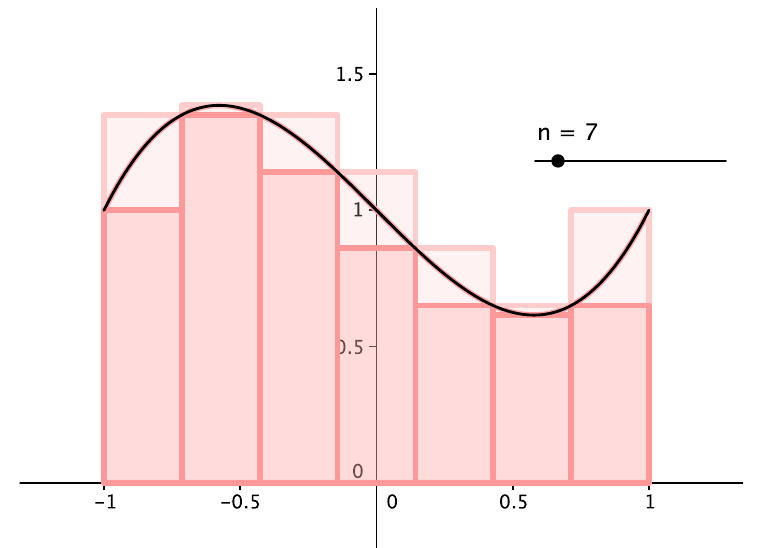
\includegraphics[width=7cm]{2020-1-C2/area-hernandez-1.png}

\newpage

...e as definições formais são:
%
$$\begin{array}{ccl}
  \mname{sup}  &=& \sumiN {\sup (f([a_i,b_i]) } \\
  \mname{inf}  &=& \sumiN {\inf (f([a_i,b_i]) } \\
\end{array}
$$

Vamos definir:
%
$$\begin{array}{ccl}
  \displaystyle \ointpx{P}{f(x)} &=& \mname{sup} \\[10pt]
  \displaystyle \uintpx{P}{f(x)} &=& \mname{inf} \\
\end{array}
$$
%
pra podermos escrever isto, ao invés de $\mname{inf} ≤
\Intx{a}{b}{f(x)} ≤ \mname{sup}$:
%
$$\displaystyle
  \uintpx{P}{f(x)} ≤
  \Intx{a}{b}{f(x)} ≤
  \ointpx{P}{f(x)}
$$

\newpage

A nossa pronúncia para estas expressões novas vai ser:

\msk

$\ointpx{P}{f(x)}$ é a ``a aproximação da integral de $f(x)$ por
retângulos por cima na particão $P$'', ou ``\ColorRed{a integral por
  cima de $f(x)$ na partição $P$}''.

\msk

$\uintpx{P}{f(x)}$ é a ``a aproximação da integral de $f(x)$ por
retângulos por baixo na particão $P$'', ou ``\ColorRed{a integral por
  baixo de $f(x)$ na partição $P$}''.

\msk

Uma das pronúncias possíveis para $\Intx{a}{b}{f(x)}$ é ``\ColorRed{a
  integral de $f(x)$ no intervalo $[a,b]$}''. Lembra que uma partição
$P$ nos dá valores para $a$ e $b$ -- $a$ é o primeiro ponto de $P$ e
$b$ é o último.

% Dizer que estamos integrando ``na partição $P$'' nos dá mais
% informação do que



\newpage

A interpretação \ColorRed{geométrica} de
%
$$\displaystyle
  \ointpx{P}{f(x)} - 
  \uintpx{P}{f(x)}
$$
%
vai ser a região em rosa claro na figura do slide 2 -- ou seja, um
\ColorRed{subconjunto de $\R^2$} formado pela \ColorRed{união} dos
\ColorRed{retângulos} em rosa claro.

\msk

A interpretação \ColorRed{numérica} da expressão acima vai ser a área
desse subconjunto. Às vezes vamos escrevê-la como:
%
$$\displaystyle
  \Area\left(
  \ointpx{P}{f(x)} - 
  \uintpx{P}{f(x)}
  \right)
$$



\newpage

% «exercicio-1»  (to ".exercicio-1")
% (c2m201defintp 6 "exercicio-1")
% (c2m201defint    "exercicio-1")

{\bf Exercício 1.} Sejam $f$ a nossa função preferida das aulas
anteriores, isto é, $f(x) = 4-(x-2)^2$, e $P = \{0,1,2,3.5\}$.

\msk

a) Represente graficamente
%
$$ \uintpx{P}{f(x)} ≤
   \Intx{a}{b}{f(x)} ≤
   \ointpx{P}{f(x)}
$$

b) Represente graficamente o conjunto $\setofst{(x,f(x))}{x∈[0,3.5]}$.

c) É verdade que 
%
$$\setofst{(x,f(x))}{x∈[0,3.5]}
  ⊆ \left(\ointpx{P}{f(x)} -
          \uintpx{P}{f(x)}
    \right) \;\; ?
$$

\newpage

% «exercicio-2»  (to ".exercicio-2")
% (c2m201defintp 7 "exercicio-2")
% (c2m201defint    "exercicio-2")

{\bf Exercício 2.}

\msk

Sejam $P_2 = \{0,1,2\}$,
      $P_3 = \{0,\frac23,\frac43,2\}$,
      $P_4 = \{0,0.5,1,1.5,2\}$.

Repare que cada $P_N$ divide o intervalo $[0,2]$ em $N$

subintervalos iguais.

Sejam $D_N = \pdintpx{P_N}{f(x)}$

para $N=2,3,4$.

\msk

a) Desenhe $D_2$ e $D_3$ de algum modo que deixe claro pro seu leitor

que $D_2 \, \ColorRed{\not\supseteq} \, D_3$.

\ssk

b) Desenhe $D_2$ e $D_4$ de algum modo que deixe claro pro seu leitor

que $D_2 \, \ColorRed{\supseteq} \, D_4$. (Dica: use um gráfico só.)

\msk

c) Defina $P_8$ e $D_8$ seguindo os padrões acima.

Desenhe $D_4$ e $D_8$ de algum modo que deixe claro pro seu leitor

que $D_4 \, \ColorRed{\supseteq} \, D_8$. (Dica: use um gráfico só.)



\newpage

% «exercicio-3»  (to ".exercicio-3")
% (c2m201defintp 8 "exercicio-3")
% (c2m201defint    "exercicio-3")

Repare que podemos escrever as partições

do intervalo $[a,b]$ em $N$ subintervalos desta forma:

\ssk

\def\atowb#1#2{a+\frac{#1(b-a)}{#2}}

$\begin{array}{ll}
 \{a,b\} & \text{(um subintervalo)} \\
 \{a,\atowb12,b\} & \text{(dois subintervalos)} \\
 \{a,\atowb13,\atowb23,b\} & \text{(três subintervalos)} \\
 \{a,\atowb14,\atowb24,\atowb34,b\} & \text{(quatro subintervalos)} \\
 \vdots & \vdots \\
 \{a,\atowb1N,\atowb2N,\ldots,b\} & \text{($N$ subintervalos)} \\
 \end{array}
$

\ssk

A \ColorRed{a nossa sequência de partições preferida para o intervalo $[a,b]$}

vai ser a sequência $(P_1, P_2, \ldots)$ na qual cada $P_k$ divide

o intervalo $[a,b]$ em $2^k$ subintervalos iguais.

\ssk

{\bf Exercício 3.} Digamos que $[a,b]=[5,12]$ e que $(P_1, P_2,
\ldots)$ seja a nossa sequência preferida de partições para este
intervalo. Calcule os três primeiros pontos de $P_4$.



\newpage

% «def-integral»  (to ".def-integral")
% (c2m201defintp 9 "def-integral")
% (c2m201defint    "def-integral")

{\bf Uma primeira definição pra integral}

\ssk

Digamos que queremos calcular $\Intx{a}{b}{f(x)}$.

Agora a função $f$ é uma função qualquer,

não necessariamente a nossa $f$ preferida,

e $[a,b]$ é um intervalo qualquer.

Seja $(P_1, P_2, \ldots)$ a nossa sequência preferida

de partições do intervalo $[a,b]$.

% Vamos definir:
% $\ointpx{}{f(x)} = \lim_{k→∞} \ointpx{P_k}{f(x)}$


\bsk



Todas estas desigualdades aqui são fáceis de visualizar:

$\begin{array}{r}
 \ointpx{P_1}{f(x)} ≥
 \ointpx{P_2}{f(x)} ≥
 \ldots ≥
 \lim_{k→∞} \ointpx{P_k}{f(x)} \\
    \begin{array}{c}
       \rotatebox{90}{$≤$} \\
       \Intx{a}{b}{f(x)} \\
       \rotatebox{90}{$≤$} \\
    \end{array} \\
 \uintpx{P_1}{f(x)} ≤
 \uintpx{P_2}{f(x)} ≤
 \ldots ≤
 \lim_{k→∞} \uintpx{P_k}{f(x)} \\
 \end{array}
$


\newpage

% «def-integral-2»  (to ".def-integral-2")

{\bf Uma primeira definição pra integral (2)}

Todas estas desigualdades aqui são fáceis de visualizar:

$\begin{array}{r}
 \ointpx{P_1}{f(x)} ≥
 \ointpx{P_2}{f(x)} ≥
 \ldots ≥
 \lim_{k→∞} \ointpx{P_k}{f(x)} \\
    \begin{array}{c}
       \rotatebox{90}{$≤$} \\
       \Intx{a}{b}{f(x)} \\
       \rotatebox{90}{$≤$} \\
    \end{array} \\
 \uintpx{P_1}{f(x)} ≤
 \uintpx{P_2}{f(x)} ≤
 \ldots ≤
 \lim_{k→∞} \uintpx{P_k}{f(x)} \\
 \end{array}
$

Nós vamos dizer que a função $f$ é \ColorRed{integrável no intervalo $[a,b]$}

se os dois limites da direita dão o mesmo resultado.

Vamos encurtar a notação um pouquinho, definindo:

$$\begin{array}{rcl}
  \ointpx{[a,b]}{f(x)} & := & \lim_{k→∞} \ointpx{P_k}{f(x)} \\
  \uintpx{[a,b]}{f(x)} & := & \lim_{k→∞} \uintpx{P_k}{f(x)} \\
  \end{array}
$$

\newpage

{\bf Uma primeira definição pra integral (3)}

\ssk

Se $\begin{array}[t]{rcl}
    \ointpx{[a,b]}{f(x)} & \ColorRed{=} & \uintpx{[a,b]}{f(x)}  \\[5pt]
       \Intx{a}{b}{f(x)} & :=           & \uintpx{[a,b]}{f(x)}. \\
    \end{array}
   $
então

\msk

Se $\begin{array}[t]{rcl}
    \ointpx{[a,b]}{f(x)} & \ColorRed{\not=} & \uintpx{[a,b]}{f(x)}    \\[5pt]
       \Intx{a}{b}{f(x)} & :=               & \ColorRed{\text{ERRO}}, \\[5pt]
    \end{array}
   $
então

e dizemos que $f$ \ColorRed{não é integrável neste intervalo}.


\bsk

Toda função $f:[a,b]→\R$ contínua é integrável em $[a,b]$.

Isto é meio óbvio visualmente -- vamos ver um esboço de uma prova
formal disso na próxima aula.


\newpage

% «exercicio-4»  (to ".exercicio-4")
% (c2m201defintp 12 "exercicio-4")
% (c2m201defint     "exercicio-4")

{\bf Uma função-escada e um exercício}

\ssk

% (find-es "tex" "cases")

Seja
%
$g(x) =
 \begin{cases}
  2 & \text{quando $x≤1$}, \\
  5 & \text{quando $1<x$}. \\
 \end{cases}
$

Seja $[a,b]=[0,3]$.

Seja $D_k = \ointpx{P_k}{g(x)} - \uintpx{P_k}{g(x)}$,

onde $(P_1, P_2, \ldots)$ é a nossa sequência de partições preferida.

\msk

{\bf Exercício 4.}

a) Desenhe o gráfico da função $g$.

b) Represente graficamente e calcule $D_2$.

c) Represente graficamente e calcule $D_3$.

d) Calcule $D_{10}$. Dicas: $D_{10}$ tem um retângulo só.

Qual é a largura da sua base? Qual é a sua altura?

Qual é a sua área?



\newpage

% «exercicio-5»  (to ".exercicio-5")
% (c2m201defintp 13 "exercicio-5")
% (c2m201defint     "exercicio-5")

{\bf Uma função não integrável}

\ssk

% (find-es "tex" "cases")

Seja
%
$h(x) =
 \begin{cases}
  2 & \text{quando $x ∈ \Q$}, \\
  5 & \text{quando $x \not∈ \Q$}. \\
 \end{cases}
$

Seja $[a,b]=[0,3]$.

Seja $D_k = \ointpx{P_k}{h(x)} - \uintpx{P_k}{h(x)}$,

onde $(P_1, P_2, \ldots)$ é a nossa sequência de partições preferida.

\msk

{\bf Exercício 5.}

a) Desenhe o gráfico da função $h$.

b) Represente graficamente e calcule $D_2$.

c) Represente graficamente e calcule $D_3$.

d) Calcule $D_{10}$.

e) Calcule $\Intx{a}{b}{h(x)}$.






%\printbibliography


% (find-latexinkscape-links "2020-1-C2/parts-preferidas-1")


\end{document}

%  __  __       _        
% |  \/  | __ _| | _____ 
% | |\/| |/ _` | |/ / _ \
% | |  | | (_| |   <  __/
% |_|  |_|\__,_|_|\_\___|
%                        
% <make>

 (eepitch-shell)
 (eepitch-kill)
 (eepitch-shell)
# (find-LATEXfile "2019planar-has-1.mk")
make -f 2019.mk STEM=2020-1-C2-def-integral veryclean
make -f 2019.mk STEM=2020-1-C2-def-integral pdf

% Local Variables:
% coding: utf-8-unix
% ee-tla: "c2m201defint"
% End:
